\documentclass[11pt]{article}

% Packages included
\usepackage[utf8]{inputenc}
\usepackage{amsmath, amssymb, amsthm}
\usepackage{tikz, pgf}
\usepackage{capt-of}
\usetikzlibrary{quotes,angles,arrows}
\usepackage{mathrsfs}
\usepackage{float}
\usepackage[nottoc]{tocbibind}
\usepackage{mathtools}
\usepackage{complexity}
\usepackage{algorithm}
%\usepackage{algorithmic}
\usepackage[noend]{algpseudocode}
\usepackage{listings}
\usepackage{minted}
\usepackage{graphicx}
\usepackage[export]{adjustbox}


% Theorems, Definitions, Corollaries etc,

\theoremstyle{theorem}
\newtheorem{theorem}{Theorem}[section]

%\theoremstyle{theorem}
%\newtheorem{lemma}[theorem]{Lemma}
 
\theoremstyle{remark}
\newtheorem*{remark}{Remark}

%\theoremstyle{note}
%\newtheorem*{note}{Note}

\theoremstyle{plain}
\newtheorem{definition}[theorem]{Definition}% reset theorem numbering for each chapter

\theoremstyle{definition}
\newtheorem{example}[theorem]{Example}

\linespread{1}

% Special operators
\DeclareMathOperator*{\Var}{\mathrm{Var}}
\DeclareMathOperator*{\Cov}{\mathrm{Cov}}
\DeclareMathOperator*{\Per}{\mathrm{Per}}

\usepackage[margin=3.5cm]{geometry}

\begin{document}
\begin{titlepage}
    \begin{center}
        \vspace*{\fill}
        
        \Huge
        \textbf{The Classical Complexity of Boson Sampling : A multi-core CPU implementation}
        
        \LARGE
        
        \vspace{2cm}
        \textbf{Manan Vaswani}
        
        \vfill
        
        Level I\\
        40cp project
        
        \vspace{0.8cm}
        
        
        \Large
        Supervisor: Dr. Rapha\"el Clifford\\
	Date: 6th May, 2019
        
    \end{center}
\end{titlepage}

\newpage
\section*{Acknowledgement of Sources}

\newpage
\tableofcontents
\newpage
\section{Introduction} %Introducing the problem and why it is interesting


\section{Background} %Background/Literature Review

\section{Preliminaries}
\subsection{Binary Gray Code} \label{sec:gray_code}

\subsection{Permanent of a matrix} \label{sec:permanent}
Computing the permanent of large matrices is one of the key parts of the Boson Sampling problem, as will be discussed in detail while explaining the problem in the subsequent sections of the paper.
\subsubsection{Definition}
\begin{definition}{\cite{marcus_minc66}}
The permanent of an $n \times n$ matrix $A = (a_{ij})$ is defined as
\begin{equation}
\Per A = \sum_{\sigma \in S_n} \prod_{i=1}^n a_{i\sigma(i)}
\end{equation}
where the sum is over all elements of the symmetric group $S_n$ i.e. over all permutations of the numbers in $[n] = \{1, 2, ... , n\}$
\end{definition}

\begin{example}
For a $2 \times 2$ matrix, the permanent is calculated as follows
\begin{equation}
\Per 
\begin{bmatrix}
a & b \\
c & d
\end{bmatrix}
= ad + bc
\end{equation}
\end{example}
\begin{example}
For a $3 \times 3$ matrix, the permanent is calculated as follows
\begin{equation}
\Per 
\begin{bmatrix}
a & b & c\\
d & e & f\\
g & h & i\\ 
\end{bmatrix}
= aei +bfg + cdh + ceg + bdi + afh
\end{equation}
\end{example}
One can observe that the definition of the permanent is similar to the more commonly used determinant function, differing in the fact that the permanent definition lacks the alternating signs. An important property to note about the permanent function is that it is invariant to transposition i.e. $\Per A = \Per A^T$ \cite{ryser_1963}.

\subsubsection{Computing the permanent}\label{prelim_permanent_calc}
Valiant showed that the problem of computing the permanent of a matrix is in the class $\# \P$-complete which implies that it is unlikely to have a polynomial time algorithm which implies that it is unlikely to have a polynomial-time algorithm \cite{valiant1979}. The naive algorithm obtained by directly translating the formula into an algorithm would run in $\mathcal{O}(n!n)$ time.

A significant improvement on the naive approach, Rysers algorithm uses a variant of the inclusion-exclusion principle and can be evaluated in $\mathcal{O}(n^2 2^n)$ time  \cite{ryser_1963}. Nijenhuis and Wilf sped this up to $\mathcal{O}(n2^n)$ time by iterating over the sum in Gray Code order \cite{Nijenhuis1978}.

Another formula that is as fast as Rysers was independently derived by Balasubramanian\cite{balasubramanian1980}, Bax\cite{bax1998}, Franklin and Bax\cite{bax1996}, and Glynn\cite{glynn2010}, all using different methods. We shall henceforth refer to this as Glynn's formula and it is described as follows.

Let $M = (m_{ij})$ be an $n \times n$ matrix with $m_{ij} \in \mathbb{C}$, then
\begin{equation}
\Per M = \frac{1}{2^{n-1}} \sum_\delta \left( \prod_{k=1}^n \delta_k \right) \prod_{j=1}^n\sum_{i=1}^n \delta_i m_{ij}
\end{equation}
where $\delta \in \{-1, 1\}^n$ with $\delta_1 = 1$. Hence there are $2^{n-1}$ such values for $\delta$.

Implementing the formula as is would require $\mathcal{O}(2^n n^2)$ time. However, iterating over the $\delta$ arrays in Gray code order reduces it to $\mathcal{O}(n 2^n)$ time.

In order to exploit this trick, let $v_j$ be the symbol used to denote the innermost sum i.e. $v_j = \sum_{i=1}^n \delta_i m_{ij}$. If $\delta$ is iterated over in Gray code order, then one can notice that the terms $\{ v_j, j \in [n]\}$ can actually be computed in $\mathcal{O}(n)$ time for a given value of $\delta$ rather than $\mathcal{O}(n^2)$ which is how long it would take if done naively. This is because successive elements of $\delta$ differ in only one position, so each successive $v_j$ differs only by the addition or subtraction of some $m_{ij}$ where $i$ is the position at which $\delta$ was last changed. Hence, the product of $v_j$ terms can now be calculated in $\mathcal{O}(n)$ time. Note that $\delta \in \{-1, 1\}^n$ but elements of the Gray code of size $n$ are in $\{0, 1\}^n$. To resolve this, map each 0 in the Gray code to a 1 of the $\delta$ array, and each 1 in the Gray Code to a -1 of the $\delta$ array.

\section{Describing the paper and specifying the problem} %Rename section
Cliiford and Clifford \cite{clifford17} gave a study and analysis of the classical complexity of the exact Boson Sampling problem and proposed an algorithm that is significantly faster than previous algorithms for the problem. The algorithm is simple to implement, and is able to solve the Boson Sampling problem for system sizes much greater than quantum computing systems currently available, which reduces the likelihood of achieving quantum supremacy in the context of Boson Sampling in the near future \textcolor{red}{rephrase last bit}.

\subsection{Explaining the problem}
A summary of the problem in purely mathematical terms is as follows. 

Let $m$ and $n$ be positive integers. Consider all possible multisets\footnote{A multiset is a special kind of set in which elements can be repeated} of size $n$ with elements in $[m]$, where $[m] = \{1, ... , m\}$. Let $z = [z_1, z_2, ... , z_n]$ be an array representation of such a multiset, with its elements in non-decreasing order. In other words, $z$ is an array of $n$ integers taken from $[m]$ (with repetition) and arranged in non-decreasing order. Define $\Phi_{m,n}$ to be the set of all distinct values that $z$ can take. Define $\mu(z) = \prod_{j=1}^m s_j !$ where $s_j$ is the multiplicity of $j$ in the array $z$ i.e. the number of times it appears in $z$.

$A = (a_{ij})$ is a complex-valued $m \times n$ matrix constructed by taking the first $n$ columns of a given $m \times m$ Haar random unitary matrix. For each $z$, build an $n \times n$ matrix $A_z$ where the $k^{\text{th}}$ row of $A_z$ is the $z_k^{\text{th}}$ row in $A$, for $k = 1, ... , n$. Finally, define a probability mass function over $\Phi_{m,n}$  as
\begin{equation}\label{boson_sampling_formula1}
q (z) = \frac{1}{\mu(z)} \left|\Per A_z \right| ^2 = \frac{1}{\mu(z)}  \left|\sum_{\sigma} \prod_{k=1}^n a_{z_k \sigma_k}\right|^2, \quad z \in \Phi_{m,n}
\end{equation}
where $\Per A_z$ is the permanent of $A_z$ and $\pi[n]$ is the set of all permutations of $[n]$.

The computing task is to simulate random samples from the above pmf $q(z)$.
\subsubsection{Calculating the size of the sample space}
The size of the sample space $ \Phi_{m,n}$ can be calculated using the `stars and bars' technique from combinatorics \cite{feller1968}. In our problem, we have $n$ `stars' representing the elements of the array $z$, and $m$ `buckets' representing all the values in $[m]$. Recall that $z$ is a sorted array representation of a multiset, so multiple `stars' can be in one `bucket'. Since there are $m$ `buckets', we need $m-1$ `bars' to divide the `stars' into `buckets'. Therefore, from a total of $m-1 + n$ objects, we need to pick $n$ of these to be the `stars'. There are $\binom{m+n-1}{n}$ ways to do this. Hence, there are $\binom{m+n-1}{n}$ possible values of $z$.

\section{The Boson Sampling Algorithm}
\subsection{The naive approach}
Translating the formula above (\ref{boson_sampling_formula1}) directly to an algorithm would require $\mathcal{O}(\binom{m+n-1}{n} n 2^n)$ time to evaluate. The $\binom{m+n-1}{n}$ term comes from the size of the sample space of the pmf, and calculating the value of the permanent using the fastest known methods takes $\mathcal{O}(n 2^n)$ time (Section \ref{prelim_permanent_calc}). With $m = \mathcal{O}(n^2)$ as suggested in \textcolor{red}{Section????}, the total running time is $\mathcal{O}(\binom{n^2+n-1}{n} n 2^n) = $ \textcolor{red}{???}. Hence, even for relatively small values of $n$ (\textcolor{red}{(give some actual numbers)}, computing the Boson Sampling problem would be intractable for even very powerful supercomputers.

In the literature \cite{clifford17}, two new algorithms are proposed for exact Boson Sampling. These are referred to as Algorithm A and Algorithm B, and both provide a significant speed up on the naive algorithm. The following subsections summarise the approach taken to obtain them.

\subsection{Algorithm A}
The approach to Algorithm A starts by expanding the sample space to a much larger size, which seems counterintuitive at first, but it allows us to express the pmf (Equation \ref{boson_sampling_formula1}) in a form that is much easier to compute. The sample space is expanded to the space of all arrays $\mathbf{r}=(r_1, r_2, ... , r_n)$ where each element $r_k$ is in $[m]$, which implies that we are considering a distribution on the product space $[m]^n$. It is stated and proved that sampling from $q(\mathbf{z})$ is equivalent to sampling from the pmf
\begin{equation} \label{eqn:algADistribution}
p(\mathbf{r}) = \frac{1}{n!} \left| \Per A_\mathbf{r} \right| ^2 = \frac{1}{n!} \left| \sum_\sigma \prod_{i=1}^n a_{r_i \sigma_i} \right| ^2 , \quad \mathbf{r} \in [m]^n 
\end{equation}
where as before, $\sigma$ is the set of all permutations of $[n]$.

This method requires $p(\mathbf{r}) = p(r_1, ... , r_n)$ to be rewritten as a product of conditional probabilities using the chain rule i.e.
\begin{equation}\label{eqn:bosonSamplingConditional}
p(\mathbf{r}) = p(r_1)p(r_2 | r_1) p (r_3 | r_1, r_2) ... p(r_n | r_1, r_2, ... , r_{n-1})
\end{equation}

We first sample $r_1$ from $p(r_1), r_1 \in [m]$. Then for $k=2, .. n$, we sample $r_k$ from the conditional pmf $p(r_k | r_1, r_2, ... , r_{k-1})$ with $r_1, ... , r_{k-1}$ fixed. After sampling all values of $r_k$, sort $(r_1, r_2, ... , r_n)$ in non-decreasing order, and that results in the array representation of a multiset sampled from the Boson Sampling distribution $q(\mathbf{z})$. In order to obtain the conditional probabilities, a formula for the joint pmf of the leading subsequences of $(r_1, ... , r_k)$ is given in Lemma 1 of the paper, and proved using arithmetic techniques and facts about probability measures. The formula in Lemma 1 is as follows:
\begin{equation}
p(r_1, ... , r_k) = \frac{(n-k)!}{n!} \sum_{c \in \mathcal{C}_k} \left| \Per A_{r_1, ... , r_k}^c \right| ^2 , \quad k = 1, ... , n
\end{equation}
where $\mathcal{C}_k$ is the set of $k-$combinations taken without replacement from $[n]$ and $A_{r_1, ... , r_k}^c$ is the matrix formed by taking only columns $c \in \mathcal{C}_k$ of the rows $(r_1, ... , r_k)$ of $A$.

Notice in equation \ref{eqn:bosonSamplingConditional}, we need to sample $r_k$ from the conditional probability distribution $p(r_k | r_1, ... , r_{k-1})$. This can be rewritten as $p(r_1, ... , r_k)/p(r_1 ... r_{k-1})$. Since $r_k$ does not appear in the denominator, in order to sample $r_k$ from the conditional pmf, we can equivalently sample from the pmf proportional to the numerator, as $(r_1, ... r_{k-1})$ are fixed, known values at this stage in the algorithm. Therefore, the formula is Lemma 1 is used to calculate the conditional pmfs at each stage, giving way to the following algorithm.

\begin{algorithm}
\caption{Boson Sampler: Single sample $\mathbf{z}$ from $q(\mathbf{z})$ in $\mathcal{O}(mn3^n)$ time}
\begin{algorithmic}[1]
\Require $m, n \in \mathbb{Z}_+$; $A$ formed by first $n$ columns of $m \times m$ Haar random unitary matrix
\State $\mathbf{r} \leftarrow \O $
\For{$k \leftarrow 1 \to n$}
\State $w_i \leftarrow \sum_{c \in \mathcal{C}_k} \left| \Per A_{(\mathbf{r}, i)}^c \right| ^2, i \in [m] $
\State $x \leftarrow \text{Sample}(w)$
\State $\mathbf{r} \leftarrow (\mathbf{r}, x)$
\EndFor
\State $\mathbf{z} \leftarrow \text{IncSort}(\mathbf{r})$
\State \textbf{return} $\mathbf{z}$
\end{algorithmic}
\end{algorithm}

The correctness of the algorithm is clear as it is simply an evaluation of the required pmf using the chain rule of probability. The literature gives a mathematical proof to derive the runtime, however here we shall give an informal explanation to obtain the runtime using the algorithm above. The runtime is dominated by the $\textbf{for}$ loop in lines 2 to 6, as the sorting step in line 7 takes only $\mathcal{O}(n \log n)$ using the fastest methods for sorting (\textcolor{red}{insert reference}). In each iteration of the $\textbf{for}$ loop, we first construct the conditional pmf on the sample space $[m]$. This is represented by a weighted array $\textbf{w}$. This involves calculating the permanents of $\left|\mathcal{C}_k\right|$ $k \times k$ matrices for each $i \in [m]$, where $k$ is the loop index variable. Sampling from this distribution (line 4) takes $\mathcal{O}(m)$ time \cite{walker1974}, but this too is dominated by the calculations in line 3, so we can ignore it. Therefore, the total time taken in the $k^\text{th}$ iteration is $\mathcal{O}(m \binom{n}{k} k 2^k)$, as $\left|\mathcal{C}_k\right| = \binom{n}{k}$ and calculating the permanent of a $k \times k$ matrix takes $\mathcal{O}(k 2^k)$ using the fastest methods. So for $n$ iterations,
\begin{equation}
\sum_{k=1}^n m k 2^k \binom{n}{k} = m \frac{2}{3} n 3^n = \mathcal{O}(mn3^n)
\end{equation}
Therefore the total time taken is $\mathcal{O}(mn3^n)$. In terms of space complexity, we only need to store one permanent calculation at a time, and the weight array for each pmf is of size $m$. These can also be stored only one at a time, so $\mathcal{O}(m)$ additional space is required.

\subsection{Algorithm B} \label{sec:algB}
The main theorem of the paper(Theorem 1) states that the time complexity of the Boson Sampling problem is $\mathcal{O}(n2^n + \text{poly}(m, n))$ where $ \text{poly}(m, n) = \mathcal{O}(mn^2)$, with $\mathcal{O}(m)$ additional space required. This is achieved using the second algorithm proposed in the paper i.e. Algorithm B.

Algorithm B makes use of the Laplace Expansion \cite{marcus_minc66} of permanents to obtain a significant speed up. The Laplace expansion allows us to calculate the permanent of a matrix using its permanent minors (the permanent of a submatrix with a column and a row removed). For any $k \times k$ matrix $B = (b_{i,j})$,
\begin{equation}
\Per B = \sum_{l=1}^k b_{k, l} \Per B_{k, l}^{\diamond},
\end{equation}
where $B_{k, l}^{\diamond}$  is the submatrix of $B$ with row $k$ and column $l$ removed. Hence the permanent of $B$ can be calculated in $\mathcal{O}(k)$ steps provided the permanent minors i.e. the values $\{ \Per B_{k, l}^{\diamond} \}$ are known.

Computing $\{ \Per B_{k, l}^{\diamond} \}$ by calculating each of the permanents independently would collectively take $\mathcal{O}(k^2 2^k)$ time as there are $k$ permanents to compute and to compute the value of each one takes $\mathcal{O}(k 2^k)$ time. Lemma 2 of the paper states that the collection $\{ \Per B_{k, l}^{\diamond} \}$ can be collectively evaluated in $\mathcal{O}(k 2^k)$ time and $\mathcal{O}(k)$ extra space. using Glynn's formula to evaluate a permanent minor for a given value of $l$, we have
\begin{equation}
\Per B_{k, l}^{\diamond} = \frac{1}{2^{k-2}} \sum_\delta \left( \prod_{i=1}^{k-1} \delta_i \right) \prod_{j \in [k] \setminus l} v_j (\delta), \quad l \in [k],
\end{equation}
where $\delta \in \{-1, 1\}^{k-1}$ with $\delta_1 = 1$ and $v_j (\delta) = \sum_{i=1}^{k-1} \delta_i b_{ij}$.
The usual trick of iterating over the values of $\delta$ in Gray code order is required to compute $\Per B_{k, l}^{\diamond}$ in $\mathcal{O}(k2^k)$ time for each value of $l$, but this would still have to be repeated $k$ times to cover all $l \in [k]$. The second and more novel trick used to achieve an additional speed up is used while calculating the products $\prod_{j \in [k] \setminus l} v_j (\delta)$. Observe that for each $l$, $\prod_{j \in [k] \setminus l} v_j (\delta) = \prod_{j \in [k]} v_j (\delta) / v_l(\delta)$. However, we cannot compute this method to compute the partial product as it would not work for cases when $v_l(\delta) = 0$. Instead, we first precompute two arrays $\mathbf{f}$ and $\mathbf{b}$ containing the forwards and backwards cumulative products of $\mathbf{v}(\delta) = (v_j(\delta), j\in [k])$ respectively as follows,
\begin{equation}
f_i = \prod_{j=1}^i v_j(\delta), \quad f_0 = 1,
\quad b_i = \prod_{j=i}^k v_j(\delta), \quad b_{k+1} = 1 \quad i \in [k].
\end{equation}
Then each partial product $\prod_{j \in [k] \setminus l} v_j (\delta)$ can be expressed as a product of two terms from $\mathbf{f}$ and $\mathbf{b}$, $f_{l-1} b_{l+1}$ for any $l \in [k]$. Since it takes $\mathcal{O}(k)$ time to compute the forward and backward cumulative product arrays and $\mathcal{O}(1)$ time to obtain each partial product $\prod_{j \in [k] \setminus l} v_j (\delta)$, for each value of $\delta$, the total time taken to simultaneously calculate the values of $\{ \Per B_{k, l}^{\diamond} \}$ is $\mathcal{O}(k2^k)$. Additional space required to store the partial products is $\mathcal{O}(k)$.

Coming back to formulating the second Boson Sampling algorithm, the sample space is now expanded even further with an auxiliary array $\mathbf{\alpha} = (\alpha_1, \alpha_2, ... , \alpha_n)$ where $\mathbf{\alpha} \in \pi(n)$, which is the set of permutation of $[n]$. The approach is similar to that of Algorithm A in that the goal is to create a succession of pmfs for leading subsequences of $\mathbf{r}$ and then progressively sampling $r_i$ from conditional pmfs on $(r_1, ... , r_{i-1})$. The conditioning variable $\mathbf{\alpha}$ helps us reformulate the pmf in such a way that we can use the permanent minors that we are able to calculate efficiently, while still ensuring that it is equivalent to sampling from the pmf $p(\mathbf{r})$ in equation \ref{eqn:algADistribution}.
Define
\begin{equation}
\phi(r_1, ... r_k | \mathbf{\alpha}) = \frac{1}{k!} \left| \Per A_{r_1, ... r_k}^{[n] \setminus \{\alpha_{k+1},  ... , \alpha_n\}} \right|^2, \quad k = 1, ... , n-1.
\end{equation}
In Lemma 3 of the paper, it is shown that $p(\mathbf{r}) = \mathbb{E}_{\mathbf{\alpha}}\{\phi(\mathbf{r} | \mathbf{\alpha})\}$, which is the expectation taken over $\mathbf{\alpha}$, uniformly distributed over $\pi(n)$ for fixed $\mathbf{r}$. The chain rule of expectation is used to prove the equality, and this full proof is provided in the literature. As in Algorithm A, a chain of conditional pmfs as follows is used,
\begin{equation} \label{eqn:algBChainRule}
\phi(\mathbf{r} | \mathbf{\alpha}) = \phi(r_1 | \mathbf{\alpha}) \phi(r_2 | r_1, \mathbf{\alpha}) \phi(r_3 | r_1, r_2, \mathbf{\alpha}) ... \phi(r_n | r_1, ... r_{n-1}, \mathbf{\alpha}), 
\end{equation}
where $\phi(r_k | r_1, ... r_{k-1}, \mathbf{\alpha}) = \phi(r_1, r_2, ... r_k | \mathbf{\alpha}) / \sum_{r_k} \phi(r_1, ... r_k | \mathbf{\alpha})$, using conditional probabilities and the law of total probability. The algorithm starts off by sampling $r_1$ from the pmf $\phi(r_1 | \mathbf{\alpha})$. Then for stages $k = 2 , ... , n$, $r_k$ is sampled from $\phi(r_k | r_1, ... r_{k-1}, \mathbf{\alpha})$ with $(r_1, ... , r_{k-1})$ fixed. Since the terms in the denominator are fixed, known values, sampling from $\phi(r_k | r_1, ... r_{k-1}$ is equivalent to sampling from the numerator, which can be evaluated by taking advantage of the Laplace Expansion of permanents. At stage $n$, the array $(r_1, ... , r_n)$ will have been sampled from $p(\mathbf{r})$. Sorting $(r_1, ... , r_n)$ in non-decreasing order gives $\mathbf{z}$, the array representation of the multiset sampled from the Boson Sampling distribution $q(\mathbf{z})$.
\begin{algorithm}
\caption{Boson Sampler: Single sample $\mathbf{z}$ from $q(\mathbf{z})$ in $\mathcal{O}(n2^n + \text{poly}(m, n))$ time}
\begin{algorithmic}[1]
\Require $m, n \in \mathbb{Z}_+$; $A$ formed by first $n$ columns of $m \times m$ Haar random unitary matrix
\State $\mathbf{r} \leftarrow \O $	\Comment{Empty array}
\State $A \leftarrow \text{Permute}(A)$	\Comment{Randomly permute columns of $A$}
\State $w_i \leftarrow \left|a_{i, 1}\right|^2, i \in [m]$	\Comment{Make indexed weighted array $w$}
\State $x \leftarrow \text{Sample}(w)$	\Comment{Sample index $x$ from $w$}
\State $\mathbf{r} \leftarrow (\mathbf{r}, x)$	\Comment{Append $x$ to $\mathbf{r}$}
\For{$k \leftarrow 2 \text{ to } n$}
\State $B_k^\diamond \leftarrow A_{\mathbf{r}}^{[k]}$
\State Compute  $\{ \Per B_{k, l}^{\diamond}, l \in [k] \}$	\Comment{From Lemma 2}
\State $w_i \leftarrow \left| \sum_{l = 1}^k \Per B_{k, l}^{\diamond} \right| ^2, i \in [m] $	\Comment{Using Laplace Expansion}
\State $x \leftarrow \text{Sample}(w)$
\State $\mathbf{r} \leftarrow (\mathbf{r}, x)$
\EndFor
\State $\mathbf{z} \leftarrow \text{IncSort}(\mathbf{r})$	\Comment{Sort $\mathbf{r}$ in non-decreasing order}
\State \textbf{return} $\mathbf{z}$
\end{algorithmic}
\end{algorithm}

Correctness holds as Algorithm B samples from successive conditional pmfs, which is equivalent to sampling from $\phi (r | \mathbf{\alpha})$ due to the chain rule of probability (Equation \ref{eqn:algBChainRule}), for a given $\mathbf{\alpha}$. Since  $\mathbf{\alpha}$ is uniformly distributed over the sample space $\pi(n)$, the algorithm equivalently samples from $\mathbb{E}_{\mathbf{\alpha}}\{\phi(\mathbf{r} | \mathbf{\alpha})\}$ which is shown to be equal to $p(r)$ in Lemma 3.

Once again, we will analyse the time complexity of the algorithm by going through the actual steps of the algorithm rather than the more mathematical explanation given in \cite{clifford17}. The time complexity of the algorithm is dominated by the \textbf{for} loop as expected. Permuting the columns of $A$ (Line 2) can be carried out in $\mathcal{O}(n)$ time using the Knuth shuffling algorithm \cite{knuth1969}. Lines 3 and 4 take $\mathcal{O}(m)$ time, in order to generate the weight array representing the pmf and sample from it. In the \textbf{for} loop from lines 6 to 11, computing the permanent minors (Line 8) takes $\mathcal{O}(k 2^k)$ time in the $k^{\text{th}}$ iteration, as discussed previously. Subsequently, the weight array in Line 9 is computed in $\mathcal{O}(mk)$ time as it is an array of size $m$, with each element taking $\mathcal{O}(k)$ time to compute as it is a sum of $k$ known terms. Sampling from this pmf takes $\mathcal{O}(m)$ time. The final sorting step outside the loop, in Line 12 takes $\mathcal{O}(n \log n)$ time, so it is dominated by the loop. Each iteration of the loop takes $\mathcal{O}(k 2^k) + \mathcal{O}(mk)$ time in total. So for all iterations, this takes
\begin{equation}
\sum_{k=2}^n \mathcal{O}(k2^k) + \mathcal{O}(mk) = \mathcal{O}(n2^n) + \mathcal{O}(mn^2)
\end{equation}
time. 

The space is dominated by the weight array in Line 9, which is of size $\mathcal{O}(m)$.

Hence, the Boson Sampling Problem can be run in $\mathcal{O}(n2^n + \text{poly}(m, n))$ time using Algorithm B.

\section{Implementation} %Describe implementation and how things are sped up

In this section, we will discuss the actual implementation of Algorithm B described above. The paper by Clifford and Clifford which demonstrated the two new algorithms is still relatively new, which explains why there have not been any open-source large scale benchmark tests for actual implementations of the algorithm.

\subsection{Original R Implementation} \label{sec:r_code}
At the time of writing this paper, the only open-source implementation is at \cite{clifford_r2017}, by the authors of the paper. The implementation is in written as a package written in R and is freely available to download and use from CRAN. This package, named `Boson Sampling' contains an implementation of Algorithm B, along with the required functions that it depends on. The relevant functions are described below.
\begin{description}
\item[\mintinline{R}{bosonSampler}] \hfill \\ The package provides a function `\mintinline{R}{bosonSampler(A, sampleSize, perm=FALSE)}', which implements the Boson Sampling Algorithm B from \cite{clifford17}. As the function definition suggests, it takes three arguments
\begin{itemize}
\item \mintinline{R}{A}: The first $n$ columns of an $m \times m$ random unitary matrix.
\item \mintinline{R}{sampleSize}: The number of independent sample values to be taken from the distribution, where each value is a vector of size $n$.
\item \mintinline{R}{perm}: Takes the value \mintinline{R}{TRUE} if the permanents and pmfs associated to each sample are required to be returned. By default, \mintinline{R}{perm=FALSE} unless specified otherwise.
\end{itemize}
Note that we do not need to explicitly provide the values $m$ and $n$ as the algorithm suggests since those values are obtained by simply checking the dimensions of the input $m \times n$ matrix using the \mintinline{R}{ncol(A)} and \mintinline{R}{nrow(A)} functions from R. This implementation allows us to obtain multiple samples from the Boson Sampling distribution using the same input matrix $A$ by repeatedly looping over the algorithm the desired number of times. One notable difference is that the input matrix $A$ is transposed right at the start, with the reason being that R stores matrices in column order so transposing the matrix makes operations easier. When accessing elements of $A$, the indices have been adjusted accordingly. Semantically, the function implements the algorithm exactly as it is, which ensures its' correctness (provided the inputs received and additional functions used are also correct).
\item[\mintinline{R}{cxPermMinors}] \hfill \\ The package provides a set of functions for computing permanents of matrices: \mintinline{R}{cxPerm(A), rePerm(B), cxPermMinors(C)}. Algorithm B requires the values $\{ \Per B_{k, l}^{\diamond}, l \in [k] \}$ to be computed in each iteration of the loop, and in order to do this, the \mintinline{R}{bosonSampler} function makes a call to the \mintinline{R}{cxPermMinors} function. This function takes an input matrix $A$ of size $k \times k-1$. Note that this is actually the transpose of the $B_k^{\diamond}$ in Line 7 of the algorithm, since the original matrix in \mintinline{R}{bosonSampler} was transposed. \mintinline{R}{cxPermMinors} is written in C\texttt{++} and is integrated into the R package using `RCpp', which is another package in R \cite{rcpp}. The package facilitates  mapping R datatypes to C\texttt{++} equivalents and vice-versa. The function also extensively uses the Armadillo package from C\texttt{++}\cite{armadillo}, which is a linear algebra library providing efficient functions and classes for vectors, matrices, and operations on them. This function calculates the permanent minors using Glynn's algorithm \cite{glynn2010} using the technique of iterating over Gray codes, by Nijenhuis and Wilf\cite{Nijenhuis1978} to iterate over Gray codes , and the trick of calculating forward and backward cumulative products described in Section \ref{sec:algB}.
\item[\mintinline{R}{randomUnitary}] \hfill \\The function \mintinline{R}{randomUnitary(size)} takes in an integer \mintinline{R}{size} as an input, and returns a $\text{size} \times \text{size}$ complex-valued random unitary matrix.
\end{description}
\subsubsection*{Example}
The function was run in the R console to produce 5 samples with $n = 10$ and $m = 100$.
\begin{minted}[frame=single,framesep=8pt]{console}
> library(BosonSampling)	# load the BosonSampling package
> set.seed(7)	# set the random seed in R
> n <- 10
> m <- 100
> A <- randomUnitary(m)[,1:n]	#construct random unitary matrix
> valueList <- bosonSampler(A, sampleSize = 5)$values
> #run Boson Sampling algorithm
> apply(valueList, 2, sort) #sort each sample
      [,1] [,2] [,3] [,4] [,5]
 [1,]    6    2    6   15    5
 [2,]    6    5    8   15   15
 [3,]   24    5    8   24   23
 [4,]   36   15   30   45   24
 [5,]   54   16   32   60   44
 [6,]   61   52   35   65   50
 [7,]   77   68   41   77   62
 [8,]   78   69   46   80   77
 [9,]   78   81   50   80   89
[10,]   79   99   52   96   95
\end{minted}

\subsection{Implementation in C\texttt{++}}
While choosing a programming language to implement a more efficient version of the Boson Sampling algorithm, performance was the key deciding factor. The language chosen was C\texttt{++} due to its reputation for speed in mathematical problems, ease of use especially for multi-threaded programs, and the availability of highly efficient linear algebra libraries such as Armadillo. As with the $R$ implementation, three core functions are required for the algorithm: a Boson Sampler (which runs the actual algorithm), a random unitary matrix generator, and a function to calculate the permanent minors of a matrix.

\paragraph{Armadillo Library:} In the implementation, we make extensive use of the C\texttt{++} Armadillo library\cite{armadillo}. Armadillo is a high quality linear algebra library that provides us with efficient implementations of matrix and vector operations. It greatly simplifies operations such as adding vectors, calculating cumulative products, and accessing matrix columns to name a few. Armadillo supports complex numbers as well, which was a necessary requirement for Boson Sampling. In addition, it supports the use of OpenMP for parallelisation, and automatically uses it in some cases to speed up computationally expensive operations.

\subsubsection{Generating a random unitary matrix}
The first step carried out was to create a function \mintinline{c++}{randomUnitary(int m)} to generate a complex-valued random unitary matrix $A$ which will be passed as an argument to the Boson Sampler. In order to generate a Haar random unitary matrix, the following algorithm from \cite{ozols2009} was used.
\begin{algorithm}
\caption{Random Unitary: Generate an $m \times m$ complex-valued random unitary matrix}
\begin{algorithmic}[1]
\Require $m \in \mathbb{Z}_+$
\State $A \leftarrow$ createRandomMatrix($m$)
\State $Q, R \leftarrow$ QRDecomposition($A$)
\State $R_{\text{diag}} \leftarrow$ Sign (Real (Diagonal ($R$)))
\State $U \leftarrow Q * R_{\text{diag}}$
\State \textbf{return} $U$
\end{algorithmic}
\end{algorithm}
QR Decomposition decomposes a given matrix $A$ into an orthogonal matrix $Q$ and a right triangular matrix $R$ such that $Q * R = A$. Armadillo provides the all the required supplementary functions used in the implementation, which made the C\texttt{++} implementation straightforward. Since this function is run only once as a preprocessing step before the Boson Sampling, extra steps to optimise or parallelise it were not taken. Firstly, because the primary aim of the project is to optimise the implementation of the Boson Sampling algorithm itself, which receives the random unitary matrix as an input, and secondly, it is already a highly efficient implementation since all the functions used are from Armadillo so have already been optimised, as mentioned before. The object returned by \mintinline{c++}{randomUnitary(int m)} is an $m \times m$ random unitary armadillo matrix.

\subsubsection{Computing the Permanent Minors} \label{sec:permMinors}
Line 8 of the algorithm requires the permanent minors of a given $k-1 \times k$ matrix to be computed. We use a separate function \mintinline{c++}{cxPermMinors(arma::cx_mat C)} which does exactly this for us. Once again, Armadillo data types and functions and data classes have been used extensively. Since the original R package (Section \ref{sec:r_code}) already had an implementation of this particular function in C\texttt{++}, we used this in our implementation to begin with and then optimised it as required. In our code, \mintinline{c++}{m} denotes number of rows and \mintinline{c++}{n} denotes number of columns of the input matrix. Since the transpose of the matrix is being used from the Boson Sampling function, \mintinline{c++}{m == n+1}. Using this notation, recall the formula for calculating the permanent minors,
\begin{equation}
\Per B_{m, l}^{\diamond} = \frac{1}{2^{m-2}} \sum_\delta \left( \prod_{s=1}^{m-1} \delta_s \right) \prod_{i \in [m] \setminus l} v_i (\delta), \quad l \in [m],
\end{equation}
where $\mathbf{\delta} \in \{-1, 1\}^{m-1}$ with $\delta_1 = 1$ and $v_i (\delta) = \sum_{j=1}^{m-1} \delta_j b_{ji}$. The two tricks to speed up the naive implementation were to iterate the values of $\mathbf{\delta}$ over the Gray code, and to compute the innermost product $\prod_{i \in [m] \setminus l} v_i (\delta), l \in [m]$ with the help of the forward and backward cumulative products (Section \ref{sec:algB}). Since there is a lot going on in this single formula, we divide the operations being performed into 5 parts for a clearer explanation:
\paragraph{a) Iterating $\mathbf{\delta}$ over Gray code:} In order to iterate over values of $\mathbf{\delta} \in \{-1, 1\}^{m-1}$ with $\delta_1 = 1$ in Gray code order (Section \ref{sec:gray_code}), the function uses the help of two additional variables, \mintinline{c++}{int j} and \mintinline{c++}{arma::ivec g}: an integer, and a vector of integers from Armadillo respectively. \mintinline{c++}{j} is the `active index' of the Gray code. In order to go from one value in the Gray code to the next, the $j^\text{th}$ bit is flipped. Additionally, the original code uses an auxiliary array \mintinline{c++}{g} to change from one value of  \mintinline{c++}{j} to the next. The condition of the \mintinline{c++}{while} loop ensures that all the Gray codes of size $n-2$ are iterated over. The $\mathbf{\delta}$ array is represented by a boolean valued vector \mintinline{c++}{d}, with \mintinline{c++}{true} being equivalent to 1, and \mintinline{c++}{false} equivalent to -1.
The relevant snippets of code from the function are shown below.
\begin{minted}[frame=lines,framesep=8pt]{c++}
int j = 0, k;
arma::uvec d(n); d.fill(true);
arma::ivec g = arma::regspace< arma::ivec>(0,(n-1));
...
while(j < n-1){
   ...
    d[j] = !d[j];
    // Iterate Gray code: j is active index
    if( j > 0){
        k = j + 1; g[j] = g[k]; g[k] = k; j = 0;
    } else {
        j = g[1]; g[1] = 1;
    }
}
\end{minted}

\paragraph{b) Computing $\mathbf{v}(\mathbf{\delta}) = \{v_i (\mathbf{\delta}), i \in [m]\}$ efficiently for each $\mathbf{\delta}$:} At the start of the function, $\mathbf{v}(\mathbf{\delta})$ is initialised to the row-sums of the input matrix \mintinline{c++}{C}, divided by two. This is because $\mathbf{\delta}$ is initialised to an all-1 (or equivalently all-\mintinline{c++}{true}) vector, so $v_i (\delta) = \sum_{j=1}^{m-1} \delta_j b_{ji} =  \sum_{j=1}^{m-1} b_{ji}$. The actual code does a row sum instead of a column sum like the formula suggests due to the matrix being transposed. The reason for dividing by 2 is explained later. In each iteration of the loop over $\mathbf{\delta}$, the active index $j$ is used to check the value of $\delta_j$, which is the element of $\mathbf{\delta}$ about to be flipped, and accordingly adds or subtracts the $j^{th}$ column to $\mathbf{v}(\mathbf{\delta})$. These operations are performed in the following lines of code.
\begin{minted}[frame=lines,framesep=8pt]{c++}
...
v = arma::sum(C,1)/2;
...
while( ... ){
    if(d[j]) v -= C.col(j); else v += C.col(j);
    ...
}
\end{minted}

\paragraph{c) Computing the partial products $\prod_{i \in [m] \setminus l} v_i (\delta), \quad l \in [m]$:} In order to exploit the trick of calculating the partial products of $\mathbf{v}(\mathbf{\delta})$ quickly, we use a vector \mintinline{c++}{p} to store the accumulated result of calculating the permanent minors, and directly add or subtract the partial products to this vector. \mintinline{c++}{p} is initialised with the partial products of the initial values of \mintinline{c++}{v} which can be seen in the lines of code that follow
\begin{minted}[frame=lines,framesep=8pt]{c++}
...
arma::cx_vec p(m), q(m);
arma::cx_double t;
...
q = arma::cumprod(v);

t = v[m-1];	// last element of v
p[m-1] = q[m-2];
for(i = m-2; i > 0; i--) {
    p[i] = t*q[i-1];
    t *= v[i];
}
p[0] = t;
...
}
\end{minted}
In this code, \mintinline{c++}{q} is the vector of forward cumulative products, and  \mintinline{c++}{t} is a single variable being used to successively store values of the backward cumulative product without having to precompute and store all of them. The same method as above is used while adding or subtracting these partial products in each iteration of the loop.

\paragraph{d) Computing the value $\left( \prod_{s=1}^{m-1} \delta_s \right)$:} Another result of iterating over $\delta$ in Gray code order is that the product $\prod_{s=1}^{m-1} \delta_s$ does not need to be calculated in each iteration of the loop. The reason being that exactly one element of $\delta$ is flipped in each iteration, so $\prod_{s=1}^{m-1} \delta_s$ alternates between the values $+1$ and $-1$ in every successive iteration. Equivalently, it means that we alternate between adding and subtracting the partial products to the accumulator in successive iterations of the loop. Therefore, this product is represented by a single boolean variable \mintinline{c++}{s} that is negated at the end of each loop iteration. %Maybe explain s being false or true.
\begin{minted}[frame=lines,framesep=8pt]{c++}
...
s = true;
...
while(j < n-1){
   ...
   if(s){
        //Subtract partial products of v from p
    } else {
        //Subtract partial products from p
    }
    s = !s;
    ...
}
\end{minted}

\paragraph{e) Multiplying by $\frac{1}{2^{m-2}}$ term:} Finally, the sum in the formula is divided by $2^{m-2}$, but rather than evaluating this separately, and dividing all the elements of the result by it, we initially divide each element of $\mathbf{v}(\mathbf{\delta})$ by 2. Then, when the partial products of $\mathbf{v}(\mathbf{\delta})$ are being computed, each partial product is divided by a factor $2^{m-1}$, and then assigned to the accumulator \mintinline{c++}{p}. Before returning  \mintinline{c++}{p} at the end of the function, it is multiplied by 2 in order to give the desired value of $2^{m-2}$ in the denominator.

The object \mintinline{c++}{p} returned is a vector containing the set of permanent minors of the input matrix \mintinline{c++}{C}.

\subsection{Simulating exact Boson Sampling using Algorithm B}
The function \mintinline{c++}{bosonSampler(arma::cx_mat A, int n, int m)} is an implementation of Algorithm B (Section \ref{sec:algB}) of the exact Boson Sampling problem in C\texttt{++}. We followed the algorithm exactly as it is, and describe a line-by-line explanation below (excluding trivial steps). The function takes as arguments a complex-valued Armadillo matrix \mintinline{c++}{A} which is a random unitary matrix as required by the algorithm, an integer \mintinline{c++}{n} representing input size, and an integer \mintinline{c++}{m} representing output modes.
\paragraph{Preprocessing steps} Before we start the actual algorithm, $A$ is required to be an $m \times n$ matrix as we require only the first $n$ columns. A random seed is generated using a Mersenne twister engine which is a uniform fast pseudo-random number generator \cite{matsumoto1998}. The random seed is required later for the sampling steps in the algorithm.
\begin{minted}[frame=lines,framesep=8pt]{c++}
// Take first n columns of A
A.set_size(m, n);

// Generate random seed
random_device rd;
mt19937 gen(rd());
\end{minted}
\paragraph{Line 2} requires the columns of $A$ to be randomly permuted. In order to do this, we have implemented a simple Knuth-shuffle algorithm \cite{knuth1969}. 
\begin{minted}[frame=lines,framesep=8pt]{c++}
// Line 2 : Permute columns
for (int i = 0; i <= n-2; i++) {
    uniform_int_distribution<int> uni(i, n-1);
    int j = uni(gen);
    A.swap_cols(i, j);
}
\end{minted}
\paragraph{Line 3 and 4} involves making a weighted array $\mathbf{w}$ and sampling a value $x$ from it. We created a C\texttt{++} standard vector of doubles to represent the weighted array using the formula provided in Line 3 of the algorithm. C\texttt{++} provides a class for creating creating discrete distributions using indexed weight arrays or vectors. This was used to generate the distribution and the random seed generated earlier was used to sample $x$ from it. 1 is added to the value sampled, as indices of C\texttt{++} vectors start at 0, but the problem requires the indices to start at 1. This sampling was carried out in the code snippet below.
\begin{minted}[frame=lines,framesep=8pt]{c++}
// Line 3
vector<double> w;
for (int i = 1; i <= m; i++) {
    w.push_back(norm(A(i-1, 1)));
}

// Line 4
discrete_distribution<> d(w.begin(), w.end());
int x = d(gen) + 1;
\end{minted}
\paragraph{Lines 6 to 11} contains the loop for repeatedly generating the marginal distributions and sampling values from them. Firstly, the permanent minors are computed of the submatrix of $A$ and stored in an Armadillo vector, by making a call to \mintinline{c++}{cxPermMinors(arma::cx_mat)}:
\begin{minted}[frame=lines,framesep=8pt]{c++}
// Line 8
arma::cx_vec perms;
perms = cxPermMinors(B_k);
\end{minted}
The permanent minors are used to create a weight vector using the formula in Line 9. As before, an integer $x$ is sampled from the discrete distribution represented by a weight vector $\mathbf{w}$, and then appended to the vector $\mathbf{r}$.
\paragraph{Line 12} is the final step of sorting the vector of sampled values $r$ in non-decreasing order. The \mintinline{c++}{sort()} function in the standard C\texttt{++} library does exactly this for vectors.
\begin{minted}[frame=lines,framesep=8pt]{c++}
// Line 12
vector<int> z;
sort(r.begin(), r.end());
z = r;
\end{minted}

\subsection{Running the code}
The files containing the functions were initially compiled on a personal computer, using the g\texttt{++} compiler with no extra flags added for optimisation. The \mintinline{c++}{main()} function required the user to enter a value of $n$ when running the function, and then set $m = n^2$. An $m \times m$ complex valued random unitary matrix is generated using the \mintinline{c++}{randomUnitary(int)} function. Subsequently, the \mintinline{c++}{bosonSampler(arma::cx_mat, int, int)} function is called, and a single sample from the Boson Sampling distribution with input size $n$ and $m$ output modes is obtained. Finally, this sample is printed out to the command line. An example of this process with $n = 10$ is shown below. The following instructions are run in the same directory as the C\texttt{++} files.
\begin{minted}[frame=single,framesep=8pt]{console}
> g++-8 bosonSampling_b_arma.cpp cxPermMinors.cpp randomUnitary.cpp \
>	 -o a.out -std=c++11 -larmadillo
> ./a.out 25
[ 7 21 28 37 38 47 63 67 91 97 ]
\end{minted}

\subsection{Profiling the code}
Once the code was running as expected, we could begin working on its efficiency and reducing the observed runtime. In order to gain a better understanding of the how the runtime of the program was divided across the functions, the Intel Vtune profiler\cite{vtune2018} was used. Code profilers dynamically analyse executable code that is running, and identify bottlenecks by giving a detailed break down of information about CPU usage, and time taken to run individual lines of the code. The profiler was run on the compiled code, and a screenshot of the results observed is shown in figure \ref{fig:vtune_hotspots_initial}.
\begin{figure}
  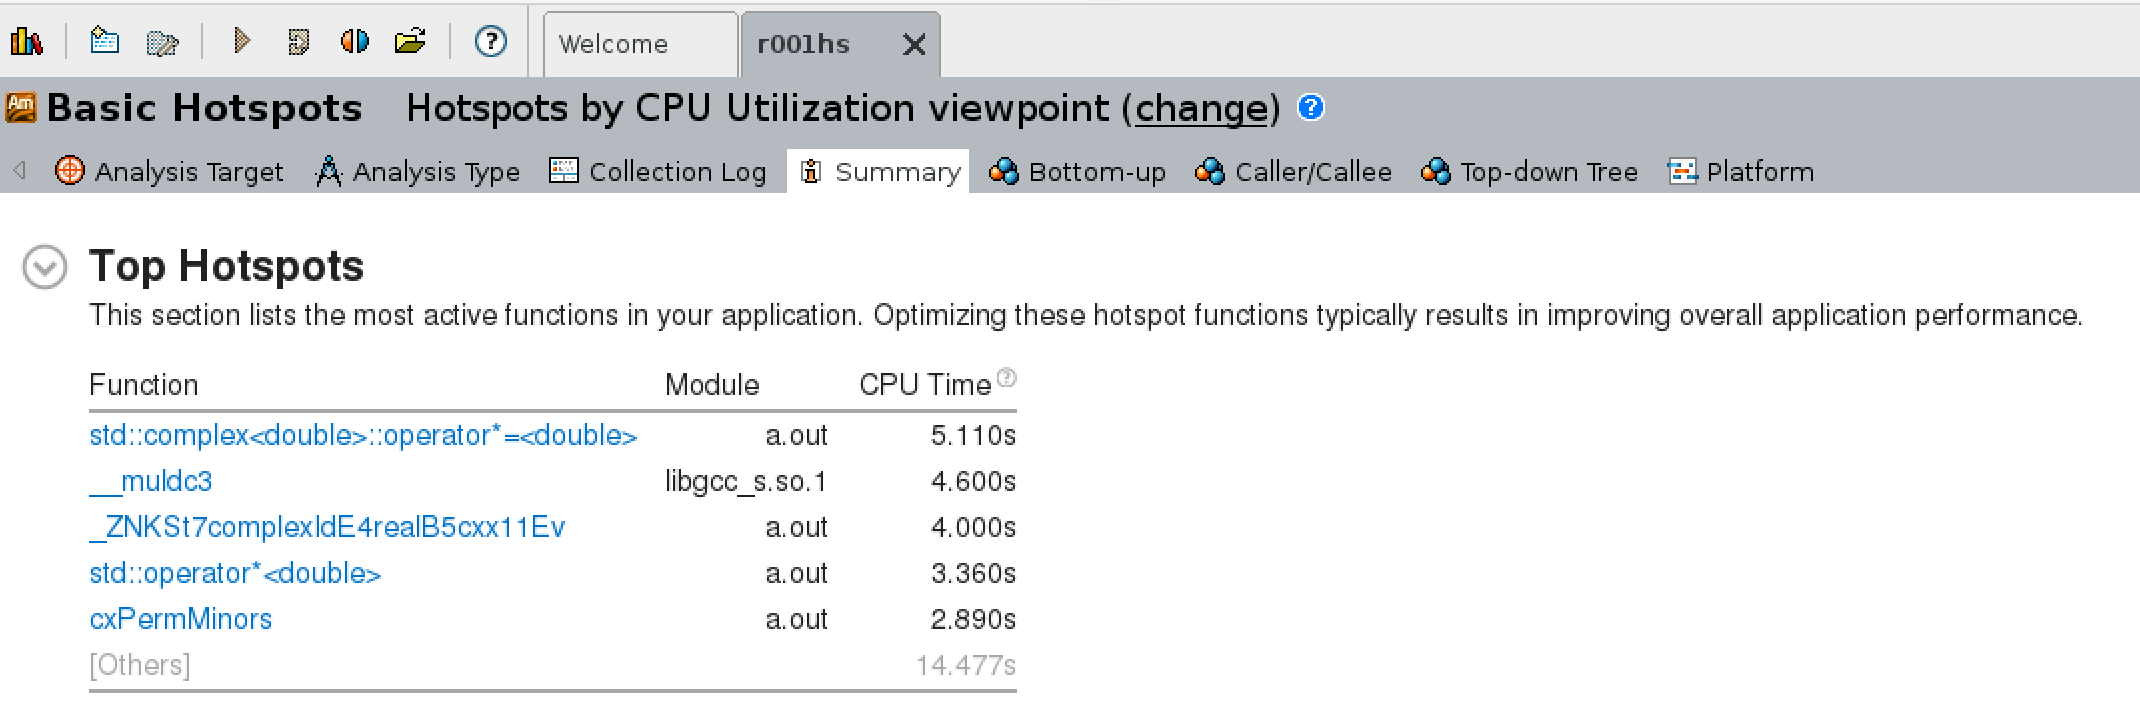
\includegraphics[width=\linewidth, frame]{vtune_hotspots_initial.png}
  \caption{A summary of `hotspots' in the code identified by the Intel Vtune Profiler}
  \label{fig:vtune_hotspots_initial}
\end{figure}
The top 4 `hotspots' identified were all related to the operation of multiplying two objects of type \mintinline{c++}{std::complex<double>}. The Bottom-Up representation within the profiler gives information on where exactly in the code the hotspots can be found. This representation showed that the top 4 hotspots were all within the \mintinline{c++}{for} loop of \mintinline{c++}{cxPermMinors( ... )}, which is exactly as expected since the runtime of the algorithm is dominated by the loop required for computing the permanent minors.

Note that the second hotspot `\_\_muldc3' is an internal library routine, which is run by the C\texttt{++} compiler when two complex numbers are multiplied. To see this, we used an online tool called GodBolt \cite{god-bolt} which converts high-level code in some programming language (C\texttt{++} in our case) to low-level, compiler-dependent assembly code that. This showed that in assembly-level language, the g\texttt{++} compiler essentially replaced lines containing the multiplication of two complex numbers with a list of instructions, one of which was `\_\_muldc3'. Complex multiplication is a fairly straightforward operation that can be simplified as follows,
\begin{equation}
(a + bi) * (c+di) = (ac - bd) + (ad + bc)i
\end{equation}
which is an operation that one would expect to be calculated very efficiently in C\texttt{++} as it is reduced to a few basic arithmetic calculations on real numbers. However, an open-source implementation of `\_\_muldc3' \cite{muldc3} shows that the function is much larger than expected, due to a number of checks being made for edge cases on complex numbers. This is another bottleneck that could potentially be resolved. The third hotspot is simply a mangled name for an internal library routine that deals with complex numbers in C\texttt{++}.

To avoid having to run the profiler every single time, a timer function was added into the code to keep track of how long the entire program takes to run, as well as the cumulative runtime of the \mintinline{c++}{cxPermMinors(...)} function.

\subsection{Parallelising the code}
\subsubsection{Parallelisation technique}
The most obvious solution to speed up the process of calculating the permanent minors is to parallelise Lines 6 to 11 of the algorithm which corresponds to the \mintinline{c++}{for} loop in the code which iterates over the values of $\delta$.For an input matrix of size $n \times n-1$, there are $(2^{n-1} -1)$ iterations of the loop. As $n$ grows, this number grows exponentially, so making the iterations run in parallel would have a significant impact. The reason that the loop is in fact parallelisable is that its purpose is essentially to generate some values in each iteration and add them to an accumulator. In order to parallelise it, each thread would have to maintain its own local accumulator, and the total number of iterations could be divided equally among the threads. After each thread completes its assigned set of iterations, it would add the values in its local accumulator to a global accumulator to a global accumulator, which would finally hold the required end result. However, this was not as trivial as it sounds since a number of variables within the loop were dependent on their values in the previous iteration. Hence, we needed to find a way to initialise these variables to the correct values for any iteration number so that a thread could be given these values to start with, and then start its set of iterations. The modifications made for this parallelisation to work are explained as follows,
\paragraph{a) Getting the value of the active index $j$ in the $k^{\text{th}}$ iteration:} The loop in the original code iterates over $\delta$ in Gray Code order by keeping track of the `active index' $j$ and then flipping the $j^{\text{th}}$ bit of $\delta$ at the end of each loop iteration. This active index $j$ is also required in calculating successive values of the vector $\mathbf{v}$, so it was also essential to derive a method for finding the value of $j$ in the $k^{\text{th}}$ iteration. To see how the value of $j$ relates to the iteration number $k$, refer to Table \ref{tab:graycode}. Notice that $j$ is equal to the position of the least significant bit set to 0 in the binary representation for $k$. Equivalently, it is the number of of trailing 0-bits in $j+1$, starting at the least significant bit position. There exists an intrinsic function (or built-in function) which does this exact operation for us. Intrinsics are a special collection of functions which are handled directly by the compiler, and are mapped directly to x86 SIMD(Single instruction, multiple data) instructions. Since these intrinsics are nearly equivalent to directly using actual assembly code, they are also highly efficient. For example, the corresponding intrinsic in the g\texttt{++} compiler is \mintinline{c++}{__builtin_ctzll (unsigned long long)}. Using this function in each iteration of the loop also allows us to get rid of the auxiliary array \mintinline{c++}{g} in the original code. it is used in the following way:
\begin{minted}[frame=lines,framesep=8pt]{c++}
int getActiveIndex(long long ctr) {
	return __builtin_ctzll(ctr);
	// _mm_tzcnt_64 for intel compiler
}
...
for (...) {
    ...
    j = getActiveIndex(ctr+1);
}
\end{minted}

\paragraph{b) Getting the value of $k^{\text{th}}$ element of the Gray code:} Once we have the correct values of $j$ in each iteration of the loop, we can use it as before to iterate from one element in the Gray code to the next in the same way as in the original implementation. However, if a thread is made to start from the $k^{\text{th}}$ iteration, it also needs to be assigned an initial value for $\delta$. Once again, refer to the example in Table \ref{tab:graycode} to see how elements of the Gray code are related to iteration number $k$. Notice that the Gray code corresponding to index $j$ is actually equal to $j \text{ XOR } j >> 1$ where $j >> 1$ represents a single bit shift to the right. \textcolor{red}{A proof of this formula by induction is shown in the appendix.} Additionally, integer representation of the Gray code element is required to be converted to the $\delta$ representation, where 1s in the Gray code are represented by 0s in $\delta$ and 0s in the Gray code are represented by 1s. The functions for these operations are called by each thread right before it starts its loop iterations.
\begin{minted}[frame=lines,framesep=8pt]{c++}
int getKthGrayCode(long long k) {
    return k ^ (k >> 1);
}
\end{minted}

\paragraph{c) Getting the value of \mintinline{c++}{s}:} Recall that \mintinline{c++}{s} was a boolean variable which decided whether partial products would be added or subtracted to the accumulator. Since in the original serial code, the value of $s$ alternated between true and false across iterations, we use the fact that for an even iteration number, \mintinline{c++}{s} was set to \mintinline{c++}{false} and for odd iterations, \mintinline{c++}{true}. This needs to be done only once for each thread, as the value of \mintinline{c++}{s} could simply be flipped at the end of each iteration to update the value correctly.
\begin{minted}[frame=lines,framesep=8pt]{c++}
//my_start is the starting index for a thread
if (my_start%2 == 0) s = false;
		else s = true;
\end{minted}

\paragraph{d) Computing the $\mathbf{v}$ array for iteration $k$:} Computing the value of $\mathbf{v}$ for a given $\delta$ requires a direct interpretation of the formula $v_i (\delta) = \sum_{j=1}^{m-1} \delta_j b_{ji}$ from the equation for calculating permanent minors. Once again, this only needs to be done once for each thread since we use a different and more efficient method to iterate from one value of $\mathbf{v}$ to the next, which was described in section \ref{sec:permMinors}.
\begin{minted}[frame=lines,framesep=8pt]{c++}
arma::cx_vec getV(arma::uvec d, int j, int n, long long ctr, arma::cx_mat C) {
    arma::cx_vec v(n);
    v = arma::sum(C,1)/2;
    for (int i = 0; i < n; i++) {
        if(d[i] == 0) v -= C.col(i);
    }
    ...
    return v;
}
\end{minted}

\begin{table}
  \begin{center}
    \caption{Elements of Gray code and active indices for $n = 4$}
    \label{tab:graycode}
    \begin{tabular}{c|c|c|c}
      \textbf{Iteration number} & $k$ \textbf{in binary} & \textbf{Active index} & \textbf{Gray code elements}\\
      $k$ & & $j$ & $\delta$\\
      \hline
      0 & 000 & 0 & 000 \\
      1 & 001 & 1 & 001 \\
      2 & 010 & 0 & 011 \\
      3 & 011 & 2 & 010 \\
      4 & 100 & 0 & 110 \\
      5 & 101 & 1 & 100 \\
      6 & 110 & 0 & 101 \\
      7 & 111 & 3 & 111 \\
    \end{tabular}
  \end{center}
\end{table}

\subsubsection{Using OpenMP to implement the code for multiple threads}

%Using the techniques discussed above, we were able to parallelise the code. Checks were run on the code and it was tested against known values of permanents of matrices to ensure correctness.




\section{Results}
\section{Further Works}
\section{Conclusion}

\bibliographystyle{unsrt}
\bibliography{project_bib}

\end{document}